\documentclass{homework}
\usepackage{enumitem}
\usepackage{tikz}
\usepackage{pgfplots}

\title{Assignment 1}
\author{
  Dmitrii, Maksimov\\
  \texttt{maksimov.dmitrii.m@gmail.com}
}
\begin{document}

\maketitle

\exercise
Let $X, Y\subseteq \R^n $ and convex, then:
\begin{enumerate}[label=\alph*)]
	\item $X\cup Y$ is not consistently convex \newline
	 \begin{figure}[!h]
		\centering
		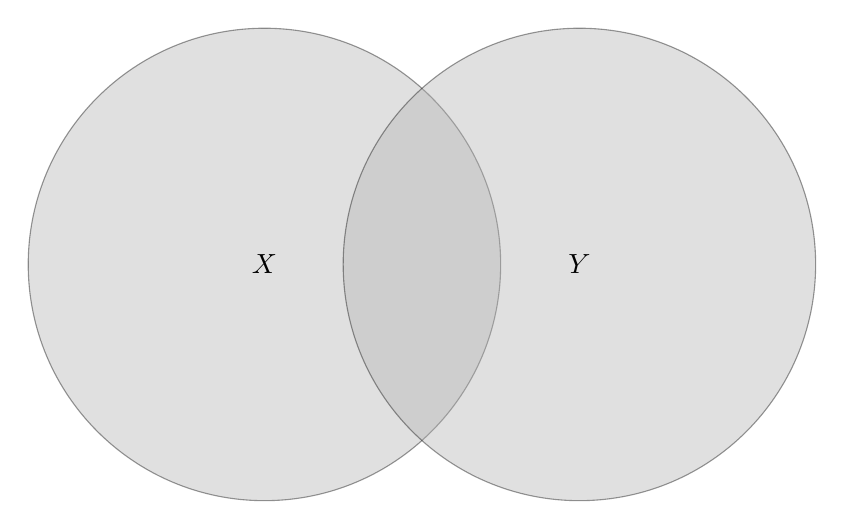
\begin{tikzpicture} [set/.style = {draw,
		    circle,
		    minimum size = 6cm,
		    fill=black!30,
		    opacity = 0.4,
		    text opacity = 1}]
		 
		\node (A) [set] {$X$};
		\node (C) at (0:4cm) [set] {$Y$};
		 
		\end{tikzpicture}
		\end{figure}
	In the set below $\exists_z: z=\alpha x + (1-\alpha) y \not\in X\cup Y$, where $x,y\in X\cup Y, \alpha \in[0,1]$
	\item $X \times Y = \{(x, y)|x\in X, y\in Y\}$ is convex \newline
	Let $(x_1, y_1), (x_2, y_2) \in X \times Y$ and $z = \alpha(x_1, y_1) + (1-\alpha)(x_2, y_2)$, then \newline$z = (\alpha x_1 + \alpha(1-\alpha)x_2, \alpha y_1 + \alpha(1-\alpha)y_2)$. Since $X,Y$ are convex, then $z\in X \times Y$
	\item $\alpha X + \beta Y = \{\alpha x+\beta y)|x\in X, y\in Y, \alpha,\beta \in \R\}$ is convex\newline
	$\alpha X$ and $\beta Y$ are affine transformations and $\alpha X + \beta Y$ is Minkowski sum. Since all of these transformations preserve convexity the result set is also convex.
	\item $\alpha X = \{\alpha x|x\in X, \alpha \in \R\}$ is convex, affine transformation
	\item $X^c=\{x\in \R^n|x\not\in X\}$ is not convex. You can imagine the complement of the $X$ from the plot above.
\end{enumerate}
Answer: a, e
\exercise*[2.1]
Let $f(x) = \log(x^TAx)$, then \newline
$\nabla f(x)=\dfrac{(A^T + A)x}{x^TAx}$. \textbf{Question: why can't we write like this: $df(x)=\dfrac{(A^T + A)xdx}{x^TAx}$? The same question for all differentials below.}

Answer: b
\exercise*[2.2]
Let $f(x) = \frac{1}{p}||x||_2^p$, then:
\begin{itemize}
	\item $\nabla f(x)=\frac{d(\frac{1}{p}(x^Tx)^{\frac{p}{2}})}{dx}=||x||_2^{p-2}x$, the gradient dimension of a scalar function is $n$ - correct
	\item $\nabla^2f(x)=\frac{d\nabla f(x)}{dx}=(p-2)||x||_2^{p-4}xx^T + ||x||_2^{p-2}I$, the hessian dimension of a scalar function is $n\times n$ - correct
\end{itemize}
\begin{enumerate}[label=\alph*)]
	\item False
	\item True
	\item False since hessian is a scalar here
	\item False
	\item True
	\item False
\end{enumerate}
Answer: b, e
\exercise*[2.3]
Let $f(x) = \frac{1}{n}\sum_{i=1}^n\log(1 + \exp(a_i^Tx)) + \frac{\mu}{2}||x||_2^2$, then:
\begin{itemize}
	\item $\nabla f(x) = \frac{1}{n}\sum_{i=1}^n\frac{\exp(a_i^Tx)}{1 + \exp(a_i^Tx)}a_i +\mu x$
	\item $\nabla^2 f(x) = \frac{1}{n}\sum_{i=1}^n\frac{\exp(a_i^Tx)(1 + \exp(a_i^Tx)a_ia_i^T - (\exp(a_i^Tx))^2a_ia_i^T}{(1 + \exp(a_i^Tx))^2} + \mu I=\frac{1}{n}\sum_{i=1}^n\frac{\exp(a_i^Tx)}{(1 + \exp(a_i^Tx))^2}a_ia_i^T + \mu I$
\end{itemize}
Answer: no, missed square in the first term
\exercise*[3]
\begin{enumerate}[label=\alph*)]
	\item $f(x)=(\sum_{i=1}^n e^{x_i})$. Since $\frac{d^n(e^x)}{dx^n}=e^x$ and $e^x > 0 \Rightarrow \nabla^2f(x)\succeq0$
	\item $f(x)=\frac{||Ax-b||^2}{1-x^Tx}$. Since $x^Tx = ||x||^2<1$, then $f(x) \geq ||Ax-b||^2. \nabla ||Ax-b||^2=2A^TA\succeq 0$, since $A^TA$ PSD matrix. the proof looks crazy :)
	\item don't know
	\item don't know if $g(x,t)=t^2 -x^Tx$ would be concave, we can prove it. This is because $-\log$ - convex, non-increasing function, but $g(x,t)$ - convex\newline
	\item From 2.3 $\nabla^2 f(x) = \frac{1}{n}\sum_{i=1}^nw_i\frac{\exp(a_i^Tx)}{(1 + \exp(a_i^Tx))^2}a_ia_i^T + \mu I$. Since eigenvalues of $a_ia_i^T \geq 0$ and other constants $\geq 0 \; \nabla^2 f(x) \succeq 0.$
	\item don't know
\end{enumerate}
\exercise*[4]
$d(f(x))=\begin{cases} 
      [-c, c],& c^Tx = 0, \\
      sign(c^Tx)c, & otherwise.
\end{cases}$
\exercise*[5]
$d(f(x))=\begin{cases} 
      [-1, 1],& x = 0, \\
      sign(x), & otherwise.
\end{cases}$
\exercise*[6]
$f(x) = ||x||_2^2 \Rightarrow \mu I\preceq\nabla^2f(x) \preceq LI\Rightarrow L=2, \mu=2$
\exercise*[3 addition]
$d(f(x))=\begin{cases} 
      (-\infty,cos(x_0)] & x = 0, \\
      \emptyset & x \in (0, x_0) \\
      cos(x) & x \in [x_0,3\pi/2) \\
      [0, +\infty) & x =3\pi/2
\end{cases}$
\end{document}